\begin{frame}{Legal Perspective: How does ML fit into the current legal framework \cite{Barocas.2016}}
US labor law (Title VII civil rights act) differentiates into \textbf{two kinds} of \textbf{discrimination}: \newline

\begin{block}{\textbf{Disparate treatment} \cite{Barocas.2016, isabel01, isabel02}}
\begin{itemize}
    \item  \textbf{Unequal behavior} towards someone because of a \textbf{protected characteristic} (\textbf{e.g.} race or gender)
    \item \underline{\textbf{ML:}} Different outputs for people with the \textbf{same values} for \textbf{non-sensitive features} but \textbf{different values} for \textbf{sensitive features}
\end{itemize}
\end{block}

\begin{block}{\textbf{Disparate impact} \cite{Barocas.2016, isabel01, isabel02}}
\begin{itemize}
    \item An equal \textbf{neutral rule} \textbf{in form}, but has a \textbf{disadvantageous effect} on some people of a protected characteristic
    \item \underline{\textbf{ML:}} Outputs benefit (hurt) people sharing a value of a protected characteristic
\end{itemize}
\end{block}
\end{frame}

\begin{frame}{Legal Perspective: How does ML fit into the current legal framework \cite{isabel01, isabel02}}
\begin{figure}
    \vspace{1cm}
    \centering
    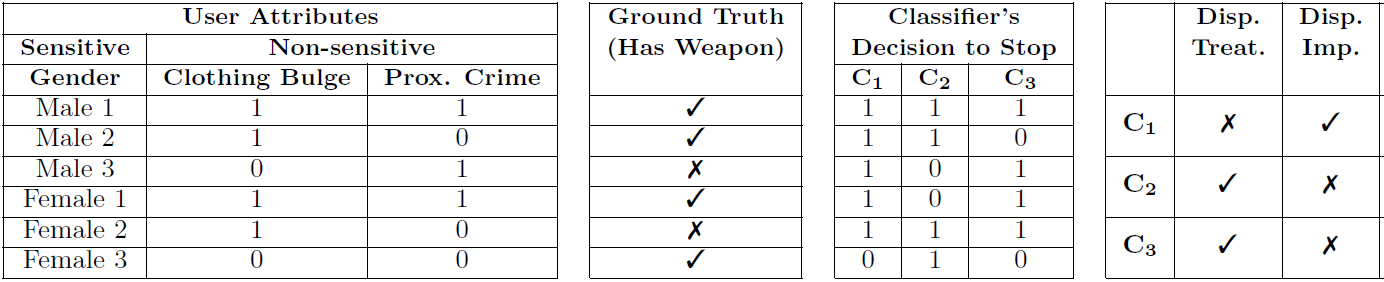
\includegraphics[width=\textwidth]{presentation/assets/DisparateTreatImp.PNG}
    \caption{Decisions of three classifiers whether (1) or not (0) to stop a pedestrian \cite{isabel01, isabel02}}
    \label{fig:exampleDisp}
\end{figure}
\end{frame}

\begin{frame}{Legal Perspective: How does ML fit into the current legal framework \cite{Barocas.2016}}
\underline{\textbf{Liability for disparate treatment:}}\\

\begin{itemize}
    \item Does not correspond to any particular discrimination mechanism within data mining
    \item Classification itself can be legal harm $\Rightarrow$ same should be true for using protected class
    \item Occurs either \textbf{at the decision} to apply a predictive, discriminatory model \textbf{OR} when the \textbf{result is used} for the hiring decision
\end{itemize}
\vspace{1cm}
\underline{\textbf{Overall:}} disparate treatment doctrine does not do much to regulate discriminatory data mining
\end{frame}

\begin{frame}{Legal Perspective: How does ML fit into the current legal framework \cite{Barocas.2016}}
\underline{\textbf{Liability for disparate impact:}}\\

\begin{itemize}
    \item Plaintiff must show that a neutral employment practice causes a disparate impact
    \item The defendant-employer may demonstrate that the practice is \textbf{job related} \& a \textbf{business necessity}
    \item Afterwards plaintiff can still show \textbf{alternative employment practice} with \textbf{less discriminatory} results
\end{itemize}
\underline{\textbf{ML:}} Threshold issue is whether or not the target variable is job related\\
\vspace{0.5cm}
$\Rightarrow$ If it's job related: 
\begin{itemize}
    \item[1.] Is the model predictive of that trait?
    \item[2.] Does the model predict what it is supposed to predict? (statistical significance showing that the result of the model correlates to the trait - extremely low bar for data mining)
\end{itemize}
\end{frame}

{
\setbeamercolor{background canvas}{bg=gray}
\begin{frame}{Legal Perspective: How does ML fit into the current legal framework \cite{Barocas.2016}}
\vspace{2cm}
\begin{block}{\huge Overall:}
\LARGE Often data mining will both \textbf{predict future job performance} and have \textbf{disparate impact} (stating a less discriminatory model is often hard)
\end{block}
\end{frame}
}

\begin{frame}{Legal Perspective: How does ML fit into the current legal framework \cite{Barocas.2016}}
    \underline{\textbf{Issues inside the data mining process:}}\\
    \begin{itemize}
        \item \textbf{Target variable} must reflect judgments about what really is the problem (\textbf{inherit bias})
        \item \textbf{Compromise} between \textbf{forbidding} employers from using past discrimination and \textbf{allowing} them to use historical data of good employees
        \item \textbf{Skewed data sets} $\Rightarrow$ type of bias, possibility to \textbf{collect more} data
        \item Not accessible data $\Rightarrow$ \textbf{oversampling} underrepresented communities
        \item \textbf{Feature selection} statistical discrimination $\Rightarrow$ \textbf{additional} or \textbf{more granular data} (else: minimizing error rates between groups)
        \item \textbf{Proxies} $\Rightarrow$ \textbf{threshold} correlation between attribute and class membership becomes alarming \& when its still relevant enough to be used
    \end{itemize}
\end{frame}